\documentclass[../../../main.tex]{subfiles}
\begin{document}

%%%%%%%%%%%%%%%%%%%%%%%%%%%%%%%%%%%%%%%%%
%%%%%%%%%%%%%%%%%%%%%%%%%%%%%%%%%%%%%%%%%
%%%%%%%%%%%%%%%%%%%%%%%%%%%%%%%%%%%%%%%%%
\chapter{Hypothesis testing and errors}

What if we make a mistake in our test, and end up making a decision that is, in fact, incorrect? How can this happen?

Well, notice that we always make a decision about the null hypothesis, and we assert either that we can, or cannot, reject it. So, if we make a mistake, it's either because: 

\begin{itemize}
  \item The null hypothesis is actually false, but we (mistakenly) conclude that we cannot reject it (so we uphold it when it is false).
  \item The null hypothesis is actually true, but we (mistakenly) conclude that we cannot accept it (so we don't uphold it when it is true).
\end{itemize}

\noindent
So there are two different types of errors that can happen. These are called \vocab{Type II} and \vocab{Type I} errors:

\begin{itemize}
  \item \vocab{Type I Error}: the null hypothesis is actually false, and we mistakenly conclude that we should leave it standing.
  \item \vocab{Type II Error}: the null hypothesis is actually true, and we mistakenly conclude that we should reject it.
\end{itemize}


%%%%%%%%%%%%%%%%%%%%%%%%%%%%%%%%%%%%%%%%%
%%%%%%%%%%%%%%%%%%%%%%%%%%%%%%%%%%%%%%%%%
\section{Type II errors}

Let's consider Type II errors first. Suppose we perform a test, and we make the decision that we cannot reject the null hypothesis. That is, we do not get enough evidence to overthrow the status quo. So the decision we make is:

\begin{center}
  Cannot reject $\NullHyp/$.
\end{center}

\noindent
We can either be right, or wrong, about this. If we're right, then $\NullHyp/$ is actually true. If we're wrong, then $\NullHyp/$ must actually be false. Think about each of these:

\begin{itemize}

  \item Consider the case where we do not get enough evidence to overthrow the null hypothesis, and so we judge that we cannot reject $\NullHyp/$, and come out thinking that the null hypothesis is (to the best of our knowledge) true. Suppose also that the null hypothesis actually is true. What then? Well, then we are making the correct decision with our test. We are concluding correctly that the null hypothesis is true, and we cannot overthrow it.

  \item Consider now the case where we do not get enough evidence to overthrow the null hypothesis, and so we do not reject it, but in fact the null hypothesis is false. What then? Well, then we are making an incorrect decision. We are concluding incorrectly that the null hypothesis is true, and we cannot overthrow it. This is a Type II error. We call it ``accepting a false null.''

\end{itemize}


%%%%%%%%%%%%%%%%%%%%%%%%%%%%%%%%%%%%%%%%%
%%%%%%%%%%%%%%%%%%%%%%%%%%%%%%%%%%%%%%%%%
\section{Type I errors}

Consider now Type I errors. Suppose we perform a test, and we make the decision that we cannot accept the null hypothesis. That is, we get enough evidence to overthrow the status quo. Then the decision we make is:

\begin{center}
  Cannot accept $\NullHyp/$.
\end{center}

\noindent
Again, we can either be right, or wrong, about this. If we're right, then $\NullHyp/$ is actually false. If we're wrong, then $\NullHyp/$ must actually be true. Think about each of these:

\begin{itemize}

  \item Consider the case where we get enough evidence to overthrow the null hypothesis, and so we judge that we cannot accept $\NullHyp/$, and come out thinking that the null hypothesis is (to the best of our knowledge) false. Suppose also that the null hypothesis actually is false. What then? Well, then we are making the correct decision with our test. We are concluding correctly that the null hypothesis is false, and we must overthrow it.

  \item Consider now the case where we get enough evidence to overthrow the null hypothesis, and so we reject it, but in fact the null hypothesis is true. What then? Well, then we are making an incorrect decision. We are concluding incorrectly that the null hypothesis is false, and we must overthrow it. This is a Type I error. We call it ``rejecting a good null.''

\end{itemize}


%%%%%%%%%%%%%%%%%%%%%%%%%%%%%%%%%%%%%%%%%
%%%%%%%%%%%%%%%%%%%%%%%%%%%%%%%%%%%%%%%%%
\section{Notation}

Here are the options, as a table:

\begin{center}
  \begin{tabular}{| l | l | l |}
    \hline
    \textbf{Decision} & \textbf{We're right} ($\NullHyp/$ is true) & \textbf{We're wrong} ($\NullHyp/$ is false) \\ \hline
    Cannot reject $\NullHyp/$ & Correct outcome & Type II error \\ \hline
    Cannot accept $\NullHyp/$ & Type I error & Correct outcome \\ \hline
  \end{tabular}
\end{center}

\noindent
There is a probability that each of these error types can occur. We call the probability of Type I errors ``alpha,'' which we symbolize with the Greek letter alpha, i.e., $\alpha$. We call the probability of Type II errors ``beta,'' which we symbolize with the Greek letter beta, i.e., $\beta$:

\begin{itemize}
  \item Probability of Type I error: $\alpha$.
  \item Probability of Type II error: $\beta$.
\end{itemize}


%%%%%%%%%%%%%%%%%%%%%%%%%%%%%%%%%%%%%%%%%
%%%%%%%%%%%%%%%%%%%%%%%%%%%%%%%%%%%%%%%%%
\section{How Type I errors happen}

Remember that we take a sample to determine if a hypothesis is correct or not. Well, what do we know about sampling? We know from the \CLT/ that the whole set of samples that can be taken from a population are always normally distributed. 

Because of this, we can draw plots of samples, and we can see exactly how Type I errors do, and do not, happen.


%%%%%%%%%%%%%%%%%%%%%%%%%%%%%%%%%%%%%%%%%
\subsection{No overlap}

Suppose we have a null hypothesis which says that the mean value of a population is 5. Like this:

\begin{equation*}
  \NullHyp/: \populationmean = 5
\end{equation*}

\noindent
To test this, we're going to have to take a sample from the population, and then generate the mean of that sample. Well, there are lots and lots of different samples we could take. But we know from the \CLT/, that all of these samples will be normally distributed. So, we can draw a picture of what all the samples would look like, on the assumption that the population mean is 5:

\begin{center}
  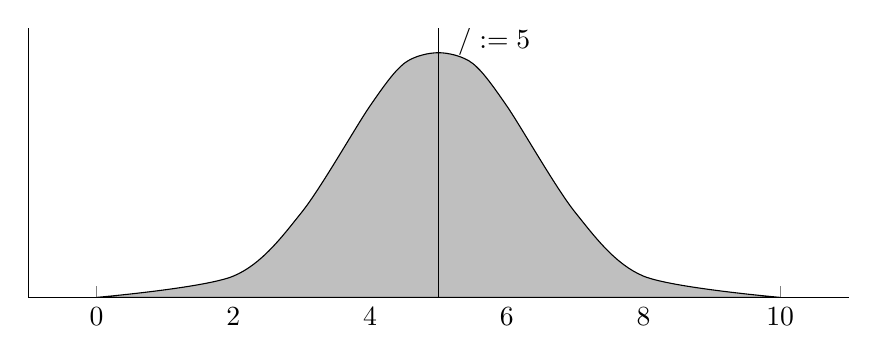
\begin{tikzpicture}
    \begin{axis}[
      axis lines*=left,
      ytick=\empty,
      height=5cm,
      width=12cm,
      enlarge y limits={value=0.1,upper},
      ]
      \addplot[smooth, fill=lightgray, domain=0:10] 
        coordinates{
          (0, 0) (2, 0.5) (3, 2) (4, 4.5) (4.5, 5.5)
          (5, 5.75)
          (5.5, 5.5) (6, 4.5) (7, 2) (8, 0.5) (10, 0)} 
        \closedcycle;
        
      \draw (5, 0) -- (5, 10);
      \node at (5, 6) [label=right:{$\NullHyp/: \populationmean = 5$}] {};

    \end{axis}
  \end{tikzpicture}
\end{center}

\noindent
What does this picture tell us? It tells us that, if the null hypothesis is true, then the real population mean is going to be 5. And then, any sample we take will have a mean that falls somewhere in the grey area. So, if we were to take a sample and calculate its mean, and then if that mean were to fall somewhere in the grey area, then that would tell us that the population mean could in fact be here the null hypothesis says it is, namely at 5.

Now let's think about the alternative hypothesis. Since the null hypothesis is $\populationmean = 5$, the alternative hypothesis will have to be $\populationmean \not = 5$. That is:

\begin{equation*}
  \AltHyp/: \populationmean \not = 5
\end{equation*}

\noindent
In other words, if the alternative hypothesis is true, then the population mean will \emph{not} be 5. What could it be? Well, it could be \emph{anything} other than 5. If the population mean is anything other than 5, then the alternative hypothesis is (in fact) true. For instance, if the population mean is 6, or 7, or even 5.00234, then the alternative hypothesis is true, because the alternative hypothesis simply says that the population mean is \emph{not} 5.

So there are an infinite number of possible sample means that would satisfy the alternative hypothesis. But for the sake of visualizing this, let's pick one. Let's suppose let the alternative hypothesis be realized be a population mean of 18. Let's mark that on our plot, like this:

\begin{center}
  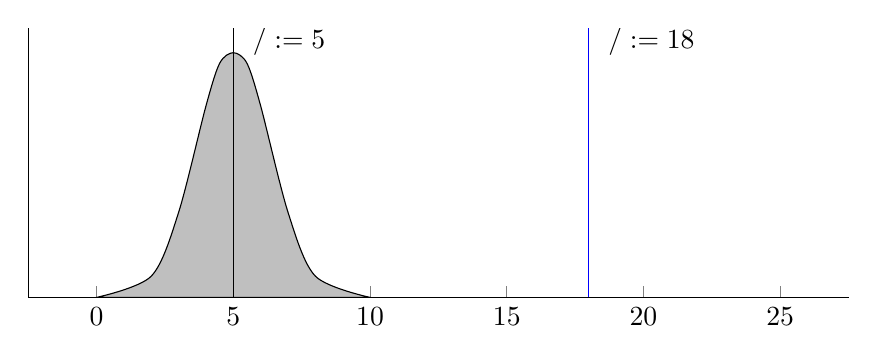
\begin{tikzpicture}
    \begin{axis}[
      axis lines*=left,
      ytick=\empty,
      height=5cm,
      width=12cm,
      enlarge y limits={value=0.1,upper},
      ]
      \addplot[smooth, fill=lightgray, domain=0:25] 
        coordinates{
          (0, 0) (2, 0.5) (3, 2) (4, 4.5) (4.5, 5.5)
          (5, 5.75)
          (5.5, 5.5) (6, 4.5) (7, 2) (8, 0.5) (10, 0)} 
        \closedcycle;
        
      \draw (5, 0) -- (5, 10);
      \node at (5, 6) [label=right:{$\NullHyp/: \populationmean = 5$}] {};

      \addplot[] coordinates{ (25, 0) };
      
      \draw[color=blue] (18, 0) -- (18, 10);
      \node at (18, 6) [label=right:{$\AltHyp/: \populationmean = 18$}] {};

    \end{axis}
  \end{tikzpicture}
\end{center}

\noindent
If the population mean were really that far to the right, then any samples we take from the population would come from around \emph{that} point. And in fact, all the samples that we could possibly take from the population would have to be normally distributed around \emph{that} point:

\begin{center}
  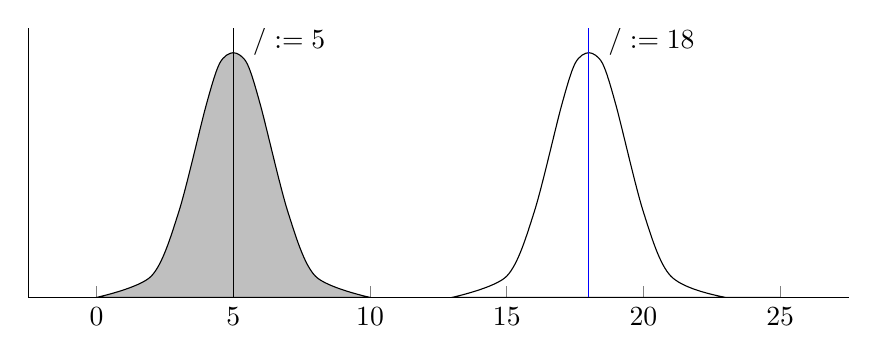
\begin{tikzpicture}
    \begin{axis}[
      axis lines*=left,
      ytick=\empty,
      height=5cm,
      width=12cm,
      enlarge y limits={value=0.1,upper},
      ]
      \addplot[smooth, fill=lightgray, domain=0:30] 
        coordinates{
          (0, 0) (2, 0.5) (3, 2) (4, 4.5) (4.5, 5.5)
          (5, 5.75)
          (5.5, 5.5) (6, 4.5) (7, 2) (8, 0.5) (10, 0)} 
        \closedcycle;
        
      \draw (5, 0) -- (5, 10);
      \node at (5, 6) [label=right:{$\NullHyp/: \populationmean = 5$}] {};

      \addplot[smooth, domain=0:30] 
        coordinates{
          (0 + 13, 0) (2 + 13, 0.5) (3 + 13, 2) (4 + 13, 4.5) (4.5 + 13, 5.5)
          (5 + 13, 5.75)
          (5.5 + 13, 5.5) (6 + 13, 4.5) (7 + 13, 2) (8 + 13, 0.5) (10 + 13, 0) (25, 0)}
        \closedcycle;

      \draw[color=blue] (18, 0) -- (18, 10);
      \node at (18, 6) [label=right:{$\AltHyp/: \populationmean = 18$}] {};

    \end{axis}
  \end{tikzpicture}
\end{center}

\noindent
What does this picture tell us? It tells us that if the population mean is really way out at 18, then any sample we can take would have a mean that falls somewhere in the white area.

Since the white and grey areas do not overlap, we know that, if the true mean were 18, there would be no way we could get a sample mean that would fall anywhere in the grey area. It would just not be possible to take a sample from the population, and get a mean that would fall anywhere near the null hypothesis's proposed mean, which is 5, if the real mean were way out at 18. 

So, if we got a sample mean that fell that far out, we would have enough evidence to reject the null hypothesis. And we would be correct to do so.

Now let's think about another case. Remember that the alternative hypothesis can be realized by an infinite number of other means (any mean that is not 5). So let's consider a case where the alternative hypothesis is realized by a value closer to the null hypothesis's proposed mean. For instance, let's think of the case where the alternative hypothesis is realized by a mean of, say, 15. Then the situation would look like this:

\begin{center}
  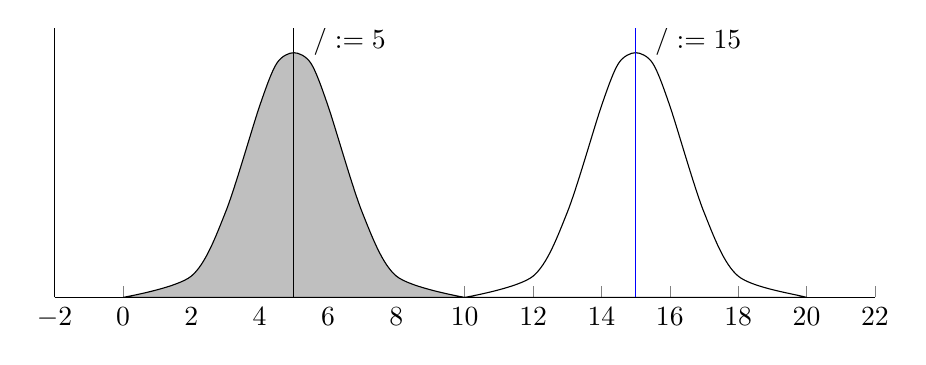
\begin{tikzpicture}
    \begin{axis}[
      axis lines*=left,
      ytick=\empty,
      height=5cm,
      width=12cm,
      enlarge y limits={value=0.1,upper},
      ]
      \addplot[smooth, fill=lightgray, domain=0:30] 
        coordinates{
          (0, 0) (2, 0.5) (3, 2) (4, 4.5) (4.5, 5.5)
          (5, 5.75)
          (5.5, 5.5) (6, 4.5) (7, 2) (8, 0.5) (10, 0)} 
        \closedcycle;
        
      \draw (5, 0) -- (5, 10);
      \node at (5, 6) [label=right:{$\NullHyp/: \populationmean = 5$}] {};

      \addplot[smooth, domain=0:30] 
        coordinates{
          (0 + 10, 0) (2 + 10, 0.5) (3 + 10, 2) (4 + 10, 4.5) (4.5 + 10, 5.5)
          (5 + 10, 5.75)
          (5.5 + 10, 5.5) (6 + 10, 4.5) (7 + 10, 2) (8 + 10, 0.5) (10 + 10, 0) (20, 0)}
        \closedcycle;

      \draw[color=blue] (15, 0) -- (15, 10);
      \node at (15, 6) [label=right:{$\AltHyp/: \populationmean = 15$}] {};

    \end{axis}
  \end{tikzpicture}
\end{center}

\noindent
In this picture, we can see that the white area is very close to the grey area, but they're not yet touching. 

So what does this picture tell us? It tells us that if the null hypothesis were correct, then the true population mean would be at 5, and any sample we took from the population would have a mean that falls somewhere in the grey area. But if the true population mean were 15, then any sample we took would have a mean that falls somewhere in the white area. 

Further, since the white and grey areas do not overlap, if the population mean really were 15, it would just not be possible to get a mean that falls anywhere near the null hypothesis's proposed mean, which is 5. So we would have enough evidence to reject the null hypothesis. And again, we would be correct to do so.

The crucial point to notice in these examples is that there is no overlap in the sampling distributions, and so if we get a sample mean that falls entirely outside of the grey area, then we know the null hypothesis's proposed mean cannot be the true population mean, so we can safely reject the null hypothesis. 


%%%%%%%%%%%%%%%%%%%%%%%%%%%%%%%%%%%%%%%%%
\subsection{Some overlap}

Again though, 18 and 15 are not the only possible means that would realize the alternative hypothesis. Let's consider a case where the curves overlap. Consider the case where the alternative hypothesis is realized by a population mean like 12. Then we'd have a picture like this:

\begin{center}
  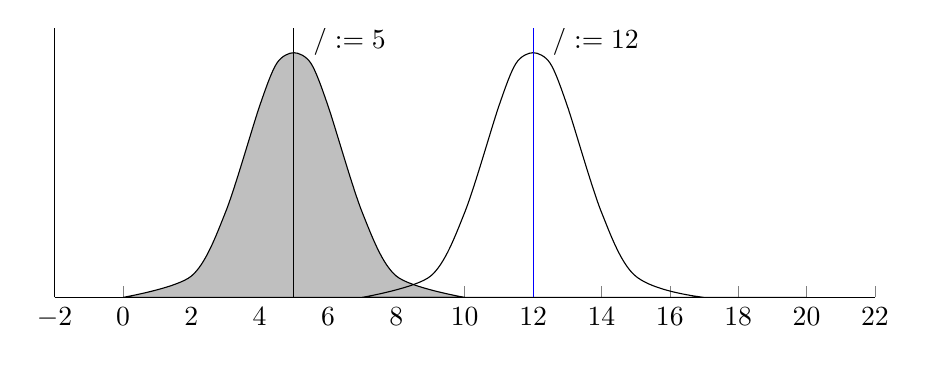
\begin{tikzpicture}
    \begin{axis}[
      axis lines*=left,
      ytick=\empty,
      height=5cm,
      width=12cm,
      enlarge y limits={value=0.1,upper},
      ]
      \addplot[smooth, fill=lightgray, domain=0:30] 
        coordinates{
          (0, 0) (2, 0.5) (3, 2) (4, 4.5) (4.5, 5.5)
          (5, 5.75)
          (5.5, 5.5) (6, 4.5) (7, 2) (8, 0.5) (10, 0)} 
        \closedcycle;
        
      \draw (5, 0) -- (5, 10);
      \node at (5, 6) [label=right:{$\NullHyp/: \populationmean = 5$}] {};

      \addplot[smooth, domain=0:30] 
        coordinates{
          (0 + 7, 0) (2 + 7, 0.5) (3 + 7, 2) (4 + 7, 4.5) (4.5 + 7, 5.5)
          (5 + 7, 5.75)
          (5.5 + 7, 5.5) (6 + 7, 4.5) (7 + 7, 2) (8 + 7, 0.5) (10 + 7, 0) (20, 0)}
        \closedcycle;

      \draw[color=blue] (12, 0) -- (12, 10);
      \node at (12, 6) [label=right:{$\AltHyp/: \populationmean = 12$}] {};

    \end{axis}
  \end{tikzpicture}
\end{center}

\noindent
Here again, we can see how samples would turn out if the population mean lived at either of these two points. 

\begin{itemize}

  \item If the population mean were at 5, as the null hypothesis proposes, then any sample mean we could take would fall somewhere in the grey area.
  
  \item if the population mean were at 12, as we see in this picture, then any sample mean we could take would fall somewhere in the white area.

\end{itemize}

\noindent
Unfortunately, there is a small area where these two curves overlap. So suppose we take a sample, and the mean of that sample happens to be 9. Let's mark that sample mean $\samplemean{x}$ on the plot with a red line:

\begin{center}
  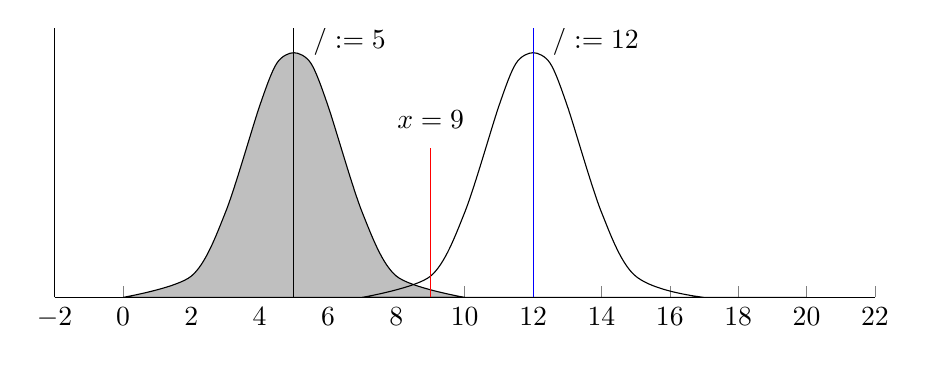
\begin{tikzpicture}
    \begin{axis}[
      axis lines*=left,
      ytick=\empty,
      height=5cm,
      width=12cm,
      enlarge y limits={value=0.1,upper},
      ]
      \addplot[smooth, fill=lightgray, domain=0:30] 
        coordinates{
          (0, 0) (2, 0.5) (3, 2) (4, 4.5) (4.5, 5.5)
          (5, 5.75)
          (5.5, 5.5) (6, 4.5) (7, 2) (8, 0.5) (10, 0)} 
        \closedcycle;
        
      \draw (5, 0) -- (5, 10);
      \node at (5, 6) [label=right:{$\NullHyp/: \populationmean = 5$}] {};

      \addplot[smooth, domain=0:30] 
        coordinates{
          (0 + 7, 0) (2 + 7, 0.5) (3 + 7, 2) (4 + 7, 4.5) (4.5 + 7, 5.5)
          (5 + 7, 5.75)
          (5.5 + 7, 5.5) (6 + 7, 4.5) (7 + 7, 2) (8 + 7, 0.5) (10 + 7, 0) (20, 0)}
        \closedcycle;

      \draw[color=blue] (12, 0) -- (12, 10);
      \node at (12, 6) [label=right:{$\AltHyp/: \populationmean = 12$}] {};

      \draw[color=red] (9, 0) -- (9, 3.5);
      \node at (9, 3.5) [label=above:{$\samplemean{x} = 9$}] {};

    \end{axis}
  \end{tikzpicture}
\end{center}

\noindent
If we get this sample mean, what can we conclude? Because the sample distributions for $\populationmean = 5$ and $\populationmean = 12$ overlap, we can't be sure which one of them our sample was taken from. Our sample could have come from either one!


%%%%%%%%%%%%%%%%%%%%%%%%%%%%%%%%%%%%%%%%%
\subsection{Making a Type I error}

Suppose that we get a sample mean of 9, and suppose that we conclude that our sample must have come from the white sampling distribution. That is to say, suppose that we accept $\AltHyp/$, and reject $\NullHyp/$.

But suppose that the null hypothesis is actually the correct. Suppose that the true population mean is 5. If that were so, we would be rejecting a good null, which is a Type I error. So here we would make a Type I error.

Can we tell if we make this error? No, not really. Remember that we simply do not know the true population mean. So, we are really just guessing here. And because these curves can overlap, that shows that it is possible for a sample to fall under two curves at the same time, and then we can get it wrong when we make our final decision. 

This example shows that it is entirely possible that we judge that the sample must come from $\AltHyp/$, when in fact it came from $\NullHyp/$. And we simply cannot know if we are right or not. Like all of inferential statistics, our final decision is just an estimate. 


%%%%%%%%%%%%%%%%%%%%%%%%%%%%%%%%%%%%%%%%%
\subsection{The probability of making a Type I error}

However, we can calculate the probability of making a Type I error. How do we do that? Well, this is yet another consequence of the \CLT/. 

Remember the empirical rule for normal distributions: 68\% of all values fall inside one standard deviation from the mean, roughly 95\% fall inside 2 deviations, and roughly 99\% fall inside 3 deviations.

The area outside of those lines, we call \vocab{alpha}, i.e., $\alpha$. So, if we are talking about 68\% of all possible values, the $\alpha$ of that is 0.32 (i.e., 32\% of the total area). If we are talking about 95\% of all possible values, the $\alpha$ of that is 0.05 (i.e., 5\% of the total area). And if we are talking about 99\% of all possible values, then the $\alpha$ of that is 0.01 (i.e., 1\% of the total area).

Let's look at $\NullHyp/$ again, but let's think of it in terms of 68\% of the values. So let's mark the extra bits in the tails outside of the 68\%:

\begin{center}
  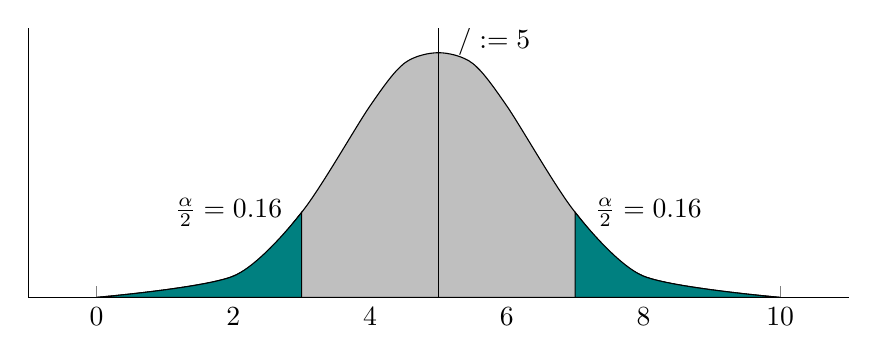
\begin{tikzpicture}
    \begin{axis}[
      axis lines*=left,
      ytick=\empty,
      height=5cm,
      width=12cm,
      enlarge y limits={value=0.1,upper},
      ]
      \addplot[smooth, fill=lightgray, domain=0:30] 
        coordinates{
          (0, 0) (2, 0.5) (3, 2) (4, 4.5) (4.5, 5.5)
          (5, 5.75)
          (5.5, 5.5) (6, 4.5) (7, 2) (8, 0.5) (10, 0)} 
        \closedcycle;
        
      \draw (5, 0) -- (5, 10);
      \node at (5, 6) [label=right:{$\NullHyp/: \populationmean = 5$}] {};

      \addplot[smooth, fill=teal, domain=0:30] 
        coordinates{
          (0, 0) (2, 0.5) (3, 2)}
        \closedcycle;

      \addplot[smooth, fill=teal, domain=0:30] 
        coordinates{
          (7, 2) (8, 0.5) (10, 0)} 
        \closedcycle;

      \node at (3, 2) [label=left:{$\frac{\alpha}{2} = 0.16$}] {};
      \node at (7, 2) [label=right:{$\frac{\alpha}{2} = 0.16$}] {};

    \end{axis}
  \end{tikzpicture}
\end{center}

\noindent
Half of the $\alpha$ is in each tail. The total area of the $\alpha$ area is 0.32 (since $1- 0.68 = 0.32$), and if you divide 0.32 in two, you get 0.16 on each side.

Now let's draw in a sampling distribution from $\AltHyp/$ now, e.g., when $\populationmean = 8$:

\begin{center}
  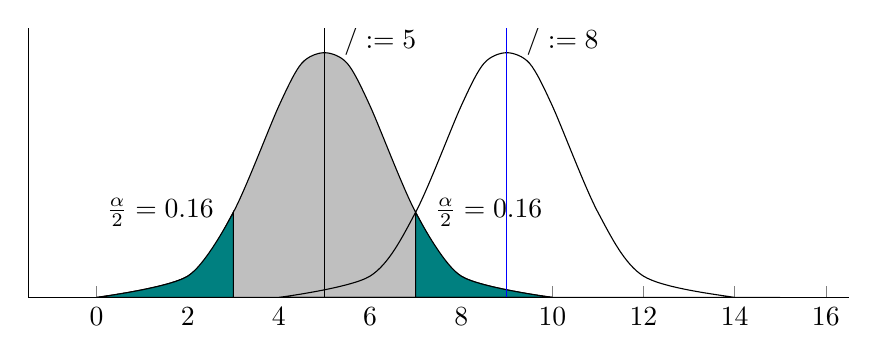
\begin{tikzpicture}
    \begin{axis}[
      axis lines*=left,
      ytick=\empty,
      height=5cm,
      width=12cm,
      enlarge y limits={value=0.1,upper},
      ]
      \addplot[smooth, fill=lightgray, domain=0:20] 
        coordinates{
          (0, 0) (2, 0.5) (3, 2) (4, 4.5) (4.5, 5.5)
          (5, 5.75)
          (5.5, 5.5) (6, 4.5) (7, 2) (8, 0.5) (10, 0)} 
        \closedcycle;
        
      \draw (5, 0) -- (5, 10);
      \node at (5, 6) [label=right:{$\NullHyp/: \populationmean = 5$}] {};

      \addplot[smooth, fill=teal, domain=0:30] 
        coordinates{
          (0, 0) (2, 0.5) (3, 2)}
        \closedcycle;

      \addplot[smooth, fill=teal, domain=0:20] 
        coordinates{
          (7, 2) (8, 0.5) (10, 0)} 
        \closedcycle;

      \node at (3, 2) [label=left:{$\frac{\alpha}{2} = 0.16$}] {};
      \node at (7, 2) [label=right:{$\frac{\alpha}{2} = 0.16$}] {};

      \addplot[smooth, domain=0:30] 
        coordinates{
          (0 + 4, 0) (2 + 4, 0.5) (3 + 4, 2) (4 + 4, 4.5) (4.5 + 4, 5.5)
          (5 + 4, 5.75)
          (5.5 + 4, 5.5) (6 + 4, 4.5) (7 + 4, 2) (8 + 4, 0.5) (10 + 4, 0) (15, 0)}
        \closedcycle;

      \draw[color=blue] (9, 0) -- (9, 10);
      \node at (9, 6) [label=right:{$\AltHyp/: \populationmean = 8$}] {};

    \end{axis}
  \end{tikzpicture}
\end{center}



\end{document}

